\documentclass[twocolumn]{article}
\usepackage[portuguese]{babel}
\usepackage[utf8]{inputenc}
\usepackage{amsmath}
\usepackage{subcaption}
\usepackage{mathtools}
\usepackage{graphicx}
\usepackage{color}
\usepackage{authblk}
\usepackage[colorlinks,citecolor=red,urlcolor=blue,bookmarks=false,hypertexnames=true]{hyperref}
\usepackage[top=15mm, bottom=15mm, left=15mm, right=15mm]{geometry}

\title{Atividade de Matemática}
\author{Prof. Leandro Vieira}
\affil{EREM Regina Pacis\\Palmerina-PE}
\date{maio de 2020}

\usepackage{lipsum}

\begin{document}

\maketitle        

\begin{enumerate}
\item Primeira de acordo com a Figura \ref{prim}

\begin{figure}[!htb]
	\centering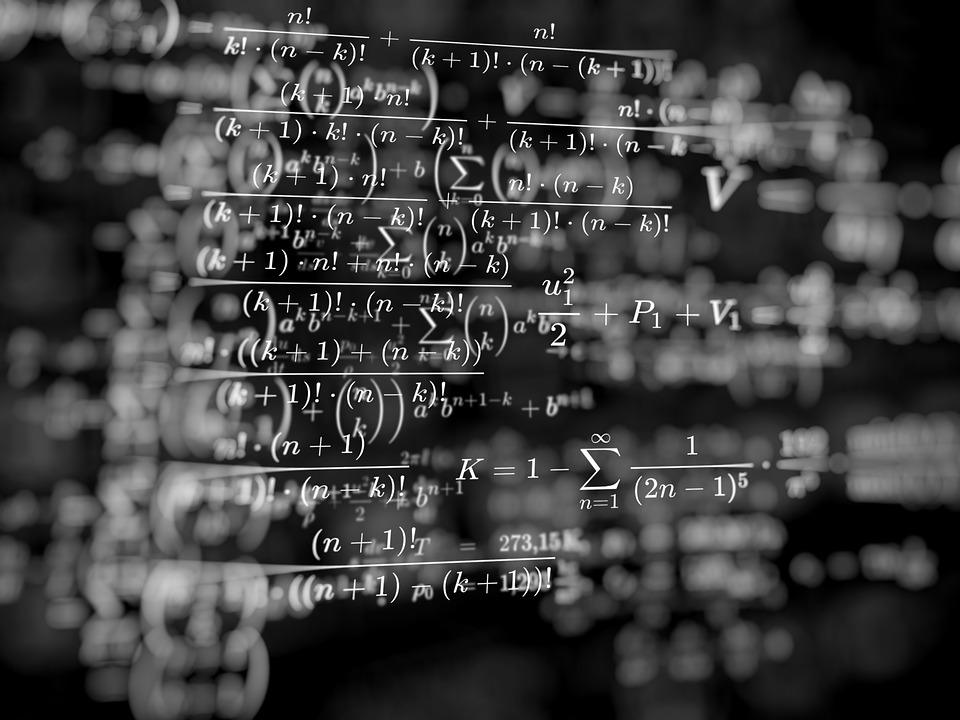
\includegraphics[width=5cm]{Figuras/imagem}\\
	\caption{Primeira}\label{prim}
\end{figure}

\item 

\begin{figure}[!htb]
	\centering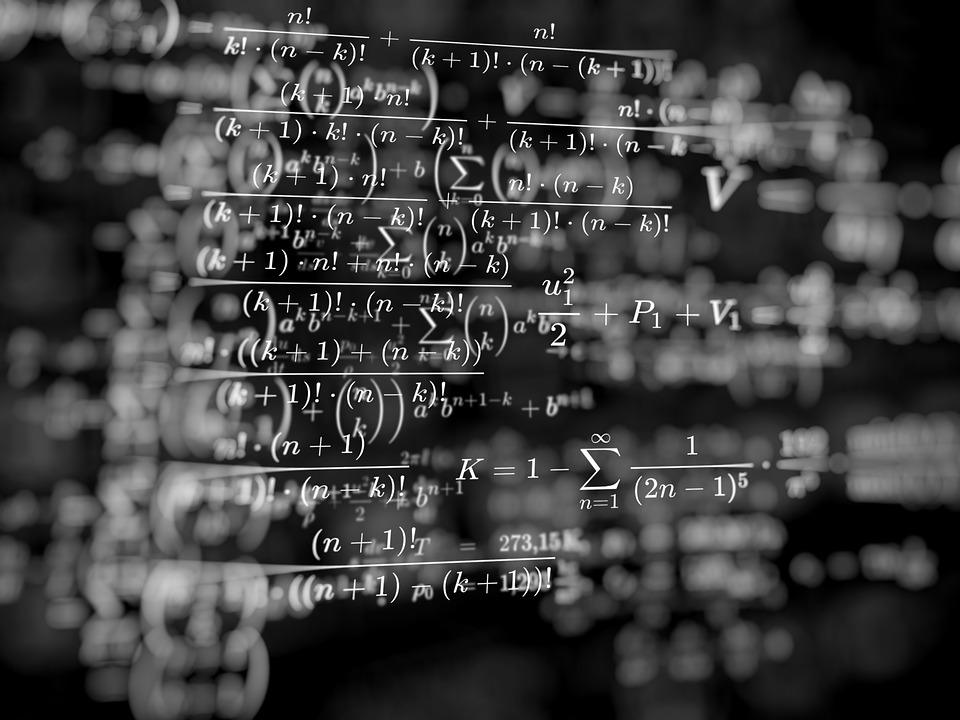
\includegraphics[width=\columnwidth]{Figuras/imagem}\\
	\caption{Segunda}\label{segunda}
\end{figure}

\end{enumerate}

\end{document}